\resizebox{0.96\textwidth}{!}{%
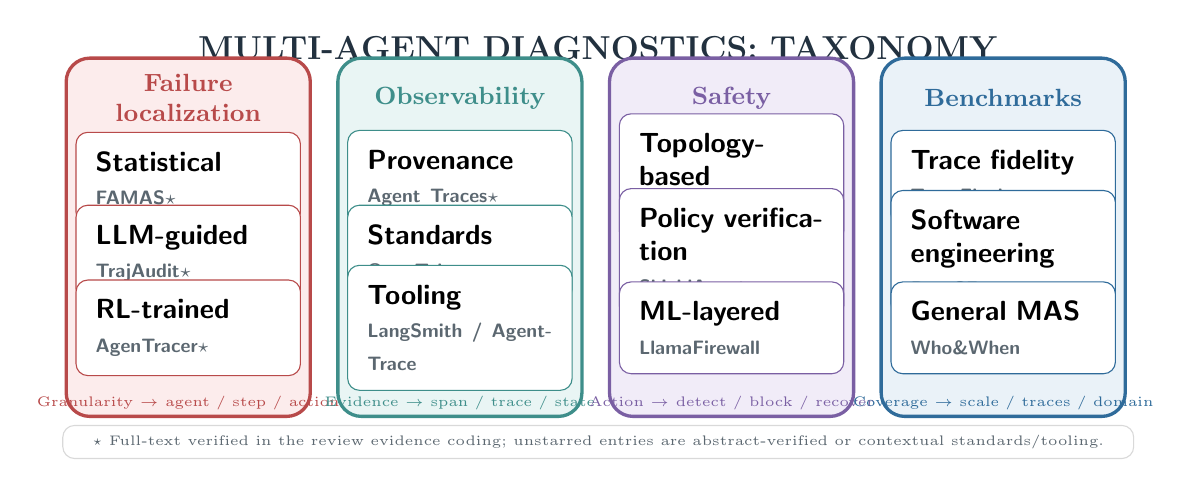
\begin{tikzpicture}[x=1cm,y=1cm,font=\sffamily]
\definecolor{cred}{HTML}{B84A4A}\definecolor{credl}{HTML}{FCECEC}
\definecolor{cteal}{HTML}{3E8E8A}\definecolor{cteall}{HTML}{E9F5F4}
\definecolor{cpurple}{HTML}{7A5FA3}\definecolor{cpurplel}{HTML}{F1ECF8}
\definecolor{cblue}{HTML}{2F6B9A}\definecolor{cbluel}{HTML}{EAF2F8}
\definecolor{cdark}{HTML}{22313F}\definecolor{cmid}{HTML}{5B6770}
\tikzset{panel/.style={rounded corners=3mm,very thick,minimum width=3.1cm,minimum height=4.55cm},
 item/.style={rounded corners=1.5mm,fill=white,minimum width=2.65cm,minimum height=0.72cm,align=left,text width=2.35cm,inner sep=2.5mm}}
\node[font=\bfseries\large,text=cdark] at (7,5.05) {MULTI-AGENT DIAGNOSTICS: TAXONOMY};
% panels
\node[panel,draw=cred,fill=credl] (p1) at (1.8,2.65) {};
\node[panel,draw=cteal,fill=cteall] (p2) at (5.25,2.65) {};
\node[panel,draw=cpurple,fill=cpurplel] (p3) at (8.70,2.65) {};
\node[panel,draw=cblue,fill=cbluel] (p4) at (12.15,2.65) {};
\node[font=\bfseries\small,text=cred,align=center] at (1.8,4.42) {Failure\\localization};
\node[font=\bfseries\small,text=cteal] at (5.25,4.42) {Observability};
\node[font=\bfseries\small,text=cpurple] at (8.70,4.42) {Safety};
\node[font=\bfseries\small,text=cblue] at (12.15,4.42) {Benchmarks};
% items
\node[item,draw=cred] at (1.8,3.40) {\bfseries Statistical\\\scriptsize\color{cmid}FAMAS$\star$};
\node[item,draw=cred] at (1.8,2.45) {\bfseries LLM-guided\\\scriptsize\color{cmid}TrajAudit$\star$};
\node[item,draw=cred] at (1.8,1.50) {\bfseries RL-trained\\\scriptsize\color{cmid}AgenTracer$\star$};
\node[item,draw=cteal] at (5.25,3.40) {\bfseries Provenance\\\scriptsize\color{cmid}Agent Traces$\star$};
\node[item,draw=cteal] at (5.25,2.45) {\bfseries Standards\\\scriptsize\color{cmid}OpenTelemetry};
\node[item,draw=cteal] at (5.25,1.50) {\bfseries Tooling\\\scriptsize\color{cmid}LangSmith / AgentTrace};
\node[item,draw=cpurple] at (8.70,3.40) {\bfseries Topology-based\\\scriptsize\color{cmid}G-Safeguard$\star$};
\node[item,draw=cpurple] at (8.70,2.45) {\bfseries Policy verification\\\scriptsize\color{cmid}ShieldAgent$\star$};
\node[item,draw=cpurple] at (8.70,1.50) {\bfseries ML-layered\\\scriptsize\color{cmid}LlamaFirewall};
\node[item,draw=cblue] at (12.15,3.40) {\bfseries Trace fidelity\\\scriptsize\color{cmid}TraceElephant$\star$};
\node[item,draw=cblue] at (12.15,2.45) {\bfseries Software\\engineering\\\scriptsize\color{cmid}RootSE$\star$};
\node[item,draw=cblue] at (12.15,1.50) {\bfseries General MAS\\\scriptsize\color{cmid}Who\&When};
\node[font=\tiny,text=cred] at (1.8,0.55) {Granularity $\rightarrow$ agent / step / action};
\node[font=\tiny,text=cteal] at (5.25,0.55) {Evidence $\rightarrow$ span / trace / state};
\node[font=\tiny,text=cpurple] at (8.70,0.55) {Action $\rightarrow$ detect / block / recover};
\node[font=\tiny,text=cblue] at (12.15,0.55) {Coverage $\rightarrow$ scale / traces / domain};
\node[draw=black!15,fill=white,rounded corners=1.5mm,minimum width=13.6cm,minimum height=0.42cm,anchor=west,font=\tiny,text=cmid] at (0.2,0.05) {$\star$ Full-text verified in the review evidence coding; unstarred entries are abstract-verified or contextual standards/tooling.};
\end{tikzpicture}%
}
